\documentclass[10pt,twocolumn,letterpaper]{article}
\usepackage[margin=0.75in,columnsep=0.25in]{geometry}
\usepackage[T1]{fontenc}
\usepackage{lmodern}
\usepackage{microtype}
\usepackage{amsmath}
\usepackage{graphicx}
\usepackage{booktabs}
\usepackage{siunitx}
\usepackage{tikz}
\usetikzlibrary{arrows.meta,positioning,fit,calc,backgrounds}
\usepackage[hidelinks]{hyperref}
\usepackage{cleveref}
\usepackage{caption}
\captionsetup{font=small,labelfont=bf}
\sisetup{detect-all,per-mode=symbol}
\graphicspath{{figs/}}
\renewcommand{\topfraction}{0.9}
\renewcommand{\dbltopfraction}{0.9}
\renewcommand{\floatpagefraction}{0.8}
\renewcommand{\dblfloatpagefraction}{0.8}
\setcounter{topnumber}{3}
\setcounter{dbltopnumber}{2}
\newcommand{\code}[1]{\texttt{\small #1}}

\title{\Large\bfseries A \SI{100}{MHz} Charge-Pump PLL with a Current-Starved Ring VCO\\
and an In-Macro TSPC Prescaler on One GF180 Tiny Tapeout Tile}
\author{ECE~298A term project, University of Waterloo\\
\small\url{https://github.com/Hive-RSI-Lab/ece298a-pll}}
\date{October 31, 2026}

\begin{document}
\maketitle

\begin{abstract}
We present a type-II, third-order charge-pump phase-locked loop (PLL) for a
single $1\times2$ Tiny Tapeout tile in the GF180MCU \SI{3.3}{V} process. A
self-biased charge pump with current steering and a rail-to-rail dump-node
buffer drives a passive second-order loop filter built from MOS capacitors;
a five-stage current-starved ring VCO with a degenerated V-to-I converter, a
floor current and a bias-tracking ceiling sets the output frequency. A
true-single-phase-clock (TSPC) divide-by-2 inside the analog macro hands the
standard-cell logic half the VCO frequency, which lifts the digital half's
worst setup slack at the slow corner from about \SI{0}{ns} to
\SI{+2.34}{ns}. The digital half (phase-frequency detector, /4 prescaler,
programmable /$N$ divider, lock detector and runaway recovery) is formally
checked, fully covered and mutation-tested. After layout and parasitic
extraction the VCO spans \SIrange{4.5}{12.9}{MHz} to
\SIrange{126}{297}{MHz} at its ends over 31 process, voltage and
temperature (PVT) corners, the loop keeps at least \SI{34.5}{\degree} of
phase margin, and a mixed-signal co-simulation of the extracted analog cell
with the hardened gate-level digital netlist and its SDF locks at
\SI{100}{MHz} ($6.25\,\text{MHz}\times16$) within \SI{6.7}{\micro s} at every
corner that bounds the range, with the control voltage settled to
\SI{14}{mV} peak-to-peak or better, and still locks with the \SI{5}{pF}
control-pad load. The tile passes DRC, LVS and the Tiny Tapeout precheck.
All of this is pre-silicon simulation: no chip has been measured. Tests
added after an outside review found the limits reported here: with the pad,
phase margin falls to \SI{23.9}{\degree}; near a corner's VCO ceiling a
divider step takes about \SI{25}{\micro s} to settle; free-running period jitter
is 10--\SI{14}{ps} rms across the corners run, not the \SI{1.2}{ps} first estimated; and under
device mismatch the charge pump's UP/DN bound fails in a quarter of samples
at its worst corner.
\end{abstract}

\section{Introduction}
Phase-locked loops are the standard way to synthesise an on-chip clock that
is a rational multiple of a reference \cite{gardner,razavi}. The charge-pump
PLL in particular gives zero static phase error with a passive filter and a
simple phase-frequency detector (PFD). This work implements one on Tiny
Tapeout's GF180 analog shuttle, which constrains the design in three ways
that shape most of the decisions below: the whole PLL, analog and digital,
must fit a $\SI{347}{}\times\SI{325}{\micro m}$ tile; Metal5 is reserved for
the shuttle, so the process's MIM capacitor (whose top plate is Metal5) is
unavailable; and the logic is built from the
\code{gf180mcu\_fd\_sc\_mcu7t5v0} standard cells, whose fastest toggle flop
is too slow, at the slow corner, to divide the VCO at its own ceiling.

The design was carried from specification to a precheck-clean GDS with open
tools only (ngspice, Magic, Netgen, KLayout, Yosys, OpenROAD/LibreLane,
Icarus Verilog, cocotb and cocotbext-ams). Every number in this paper is
taken from a result recorded in the repository, and every figure is
regenerated from those records by \code{docs/paper/make\_figs.py}.

\Cref{sec:arch} gives the architecture and frequency plan,
\cref{sec:analog} the analog circuits, \cref{sec:digital} the digital half,
\cref{sec:loop} the loop dynamics, \cref{sec:phys} the physical design,
\cref{sec:results} the post-layout and closed-loop results, and
\cref{sec:disc} the limitations.

\section{Architecture}\label{sec:arch}

\begin{figure*}[t]
\centering
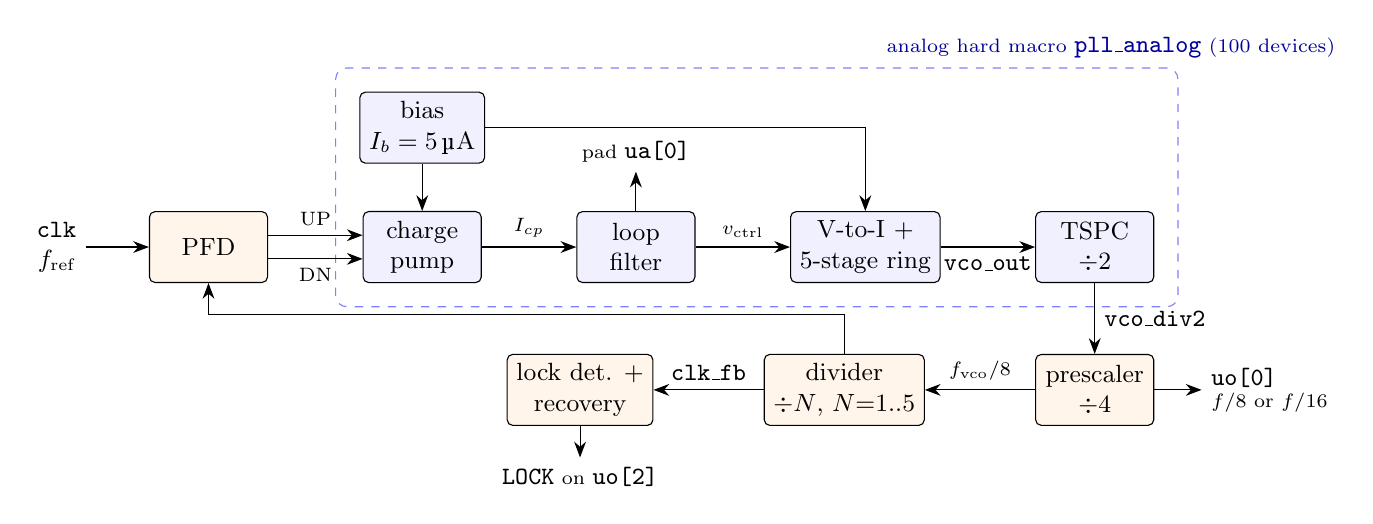
\begin{tikzpicture}[
  >={Stealth[length=2mm]}, font=\small,
  blk/.style={draw, rounded corners=2pt, minimum height=9mm, minimum width=15mm, align=center, fill=white},
  ana/.style={blk, fill=blue!6}, dig/.style={blk, fill=orange!8}]
\node[dig] (pfd) {PFD};
\node[ana, right=12mm of pfd] (cp) {charge\\pump};
\node[ana, right=12mm of cp] (lf) {loop\\filter};
\node[ana, right=12mm of lf] (vco) {V-to-I +\\5-stage ring};
\node[ana, right=12mm of vco] (tspc) {TSPC\\$\div 2$};
\node[dig, below=9mm of tspc] (pre) {prescaler\\$\div 4$};
\node[dig, left=14mm of pre] (div) {divider\\$\div N$, $N{=}1..5$};
\node[dig, left=14mm of div] (lock) {lock det. +\\recovery};
\node[ana, above=6mm of cp] (bias) {bias\\$I_b = \SI{5}{\micro A}$};
\node[left=8mm of pfd, align=center] (ref) {\code{clk}\\$f_\text{ref}$};
\draw[->] (ref) -- (pfd);
\draw[->] ([yshift=1.5mm]pfd.east) -- node[above,font=\scriptsize]{UP} ([yshift=1.5mm]cp.west);
\draw[->] ([yshift=-1.5mm]pfd.east) -- node[below,font=\scriptsize]{DN} ([yshift=-1.5mm]cp.west);
\draw[->] (cp) -- node[above,font=\scriptsize]{$I_{cp}$} (lf);
\draw[->] (lf) -- node[above,font=\scriptsize]{$v_\text{ctrl}$} (vco);
\draw[->] (vco) -- node[below,font=\scriptsize]{\code{vco\_out}} (tspc);
\draw[->] (tspc) -- node[right,font=\scriptsize]{\code{vco\_div2}} (pre);
\draw[->] (pre) -- node[above,font=\scriptsize]{$f_\text{vco}/8$} (div);
\draw[->] (div) -- node[above,font=\scriptsize]{\code{clk\_fb}} (lock);
\draw[->] (div.north) |- ($(pfd.south)+(0,-4mm)$) -- (pfd.south);
\draw[->] (bias) -- (cp);
\draw[->] (bias) -| (vco);
\draw[->] (lf.north) -- ++(0,5mm) node[above,font=\scriptsize,align=center]{pad \code{ua[0]}};
\draw[->] (pre.east) -- ++(6mm,0) node[right,font=\scriptsize,align=left]{\code{uo[0]}\\$f/8$ or $f/16$};
\draw[->] (lock.south) -- ++(0,-4mm) node[below,font=\scriptsize]{\code{LOCK} on \code{uo[2]}};
\begin{scope}[on background layer]
\node[draw=blue!50, dashed, rounded corners, inner sep=3mm, fit=(cp)(lf)(vco)(tspc)(bias),
  label={[blue!60!black,font=\scriptsize]above right:analog hard macro \code{pll\_analog} (100 devices)}] {};
\end{scope}
\end{tikzpicture}
\caption{Block diagram. Blue: the transistor-level analog macro. Orange:
standard-cell logic. Locked, $f_\text{vco} = 8N f_\text{ref}$.}
\label{fig:block}
\end{figure*}

\Cref{fig:block} shows the loop. The reference on \code{clk}
(\SIrange{5}{12.5}{MHz}) and the divided VCO clock \code{clk\_fb} drive a
tri-state PFD, whose UP and DN pulses switch the charge pump into the loop
filter. The filter voltage $v_\text{ctrl}$ sets the ring VCO's frequency.
The VCO is divided by 2 in the analog macro, by 4 in a ripple prescaler and
by a programmable $N\in\{1,\dots,5\}$, so
\begin{equation}
  f_\text{vco} = 8N\,f_\text{ref},\qquad P = 8.
\end{equation}
The nominal operating point used for every closed-loop test is
$f_\text{ref} = \SI{6.25}{MHz}$, $N=2$ ($PN=16$), $f_\text{vco} =
\SI{100}{MHz}$. Six digital signals cross between the halves
(\code{vco\_div2}, \code{pfd\_up}, \code{pfd\_dn}, \code{pll\_en},
\code{cp\_trim[1:0]}); $v_\text{ctrl}$ and an optional external bias
resistor reach the analog pads \code{ua[0]} and \code{ua[1]}.

\section{Analog design}\label{sec:analog}
The macro holds 100 devices in eight blocks: an enable inverter, the bias,
the charge pump with its dump-node buffer, the loop filter, the V-to-I
converter, the ring, the output buffer and the TSPC divider. All
transistors are \SI{3.3}{V} \code{nfet\_03v3}/\code{pfet\_03v3}; resistors
are unsalicided P+ poly (\code{ppolyf\_u}).

\subsection{Bias}
A $V_{GS}/R$ self-biased reference sets $I_b = V_{GS,B1}/R_\text{bias}
\approx \SI{5}{\micro A}$ with $R_\text{bias}\approx\SI{180}{k\ohm}$.
Biasing $M_{B1}$ near its zero-temperature-coefficient current density
leaves the resistor's tempco as the main temperature dependence. Because
the reference's loop also contains a positive-feedback path through the
PMOS mirror, a pad capacitance placed directly on the loop node made it
relax (a \SI{1.3}{\micro s} sawtooth in simulation). Splitting the resistor
so that $R_\text{top}$ isolates the loop node from the pad keeps the input
admittance's real part positive for any pad capacitance once
$g_{m1}g_{m2}R_\text{top}^2 > 1$. A start-up branch releases once the
reference conducts; at \code{ss\_m40c\_vm10} it needed $L=\SI{4}{\micro m}$
on the release transistor to avoid a second operating point.

\subsection{Charge pump}
The pump current is a trimmed mirror of $I_b$,
\begin{equation}
I_{cp} = (4 + t_0 + 2t_1 + t_0t_1)\,I_b = 20/25/30/\SI{40}{\micro A},
\end{equation}
shared by the UP source and DN sink. Long-channel ($L = \SI{2}{\micro m}$)
source and sink devices keep UP/DN mismatch low over
$v_\text{ctrl}\in[0.3, V_{DD}-0.3]$. Current steering keeps both sources
always on: when idle their current flows into a dump node that a
complementary-input, rail-to-rail unity-gain OTA holds at $v_\text{ctrl}$,
so a switch event finds its source node already at the output voltage and
injects little charge. Without the buffer, the floating dump node gave
\SI{25}{fC} of net charge per event against a \SI{10}{fC} bound; with it the
worst case over 31 corners is \SI{3.6}{fC} (\cref{fig:cp}b).

\begin{figure*}[t]
\centering
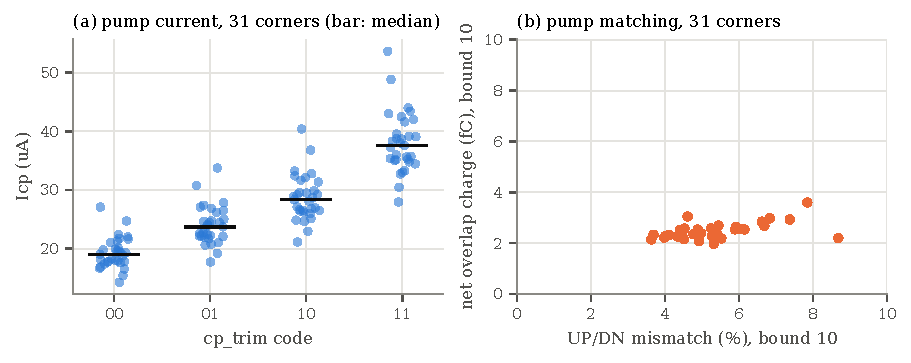
\includegraphics[width=\textwidth]{chargepump}
\caption{Charge pump over the 31 PVT corners (schematic). (a) UP current
per trim code; the code-11/code-00 ratio is 1.96--1.98 at every corner.
(b) UP/DN mismatch at code 00 against net overlap charge, both within their
\SI{10}{\%} and \SI{10}{fC} bounds.}
\label{fig:cp}
\end{figure*}

\subsection{Loop filter}
The filter is the classic series $R_1C_1$ with a shunt $C_2$:
\begin{equation}
Z(s) = \frac{1+sR_1C_1}{s(C_1+C_2)\left(1+sR_1\frac{C_1C_2}{C_1+C_2}\right)},
\end{equation}
with $R_1\approx\SI{27}{k\ohm}$ (a \SI{150}{\micro m} poly resistor),
$C_1 = \SI{20.1}{pF}$ and $C_2 = \SI{2.1}{pF}$. These place the zero at
\SI{293}{kHz} and the pole at \SI{3.06}{MHz}. Since Tiny Tapeout's GF180
stack forbids Metal5, both capacitors are \code{cap\_nmos\_03v3\_b}
accumulation-mode MOS capacitors (about \SI{3.98}{fF/\micro m^2} at
\SI{1.6}{V}) in place of MIM: $C_1$ is twelve $35\times\SI{12}{\micro m}$
units. The MOS capacitor loses about \SI{9}{\%} of its value near
$v_\text{ctrl}=\SI{0.3}{V}$, which only affects the lowest output
frequencies. Moving from MIM to MOS shifted phase margin by
$+0.1$ to $+0.3^\circ$ and the post-layout VCO by at most about \SI{1}{\%}.

\subsection{VCO}
The control voltage drives a source-degenerated V-to-I converter,
\begin{equation}
I_\text{ctl} = I_\text{floor} + \frac{v_\text{ctrl}-V_{TH}-V_S}{R_\text{V2I}},
\end{equation}
whose current is mirrored into the PMOS and NMOS starving rails of a
five-stage inverter ring, giving $f \approx I_\text{ctl}/(5\,C_\text{node}V_{DD})$.
Two additions bound the range. A floor current (a copy of $I_b$) keeps the
ring oscillating at $v_\text{ctrl}=\SI{0.3}{V}$. A ceiling device in series
with $R_\text{V2I}$, also mirrored from $I_b$, saturates at high
$v_\text{ctrl}$ and caps $f_\text{max}$; without it the ring reached
390--\SI{400}{MHz} at the fast, cold, high-supply corner. A NAND with
\code{pll\_en} and an inverter buffer the ring to full swing with
\SIrange{0.03}{0.07}{ns} edges and a \SIrange{53}{55}{\%} duty cycle.
\Cref{fig:vco} shows the extracted VCO's tuning curves.

\begin{figure}[t]
\centering
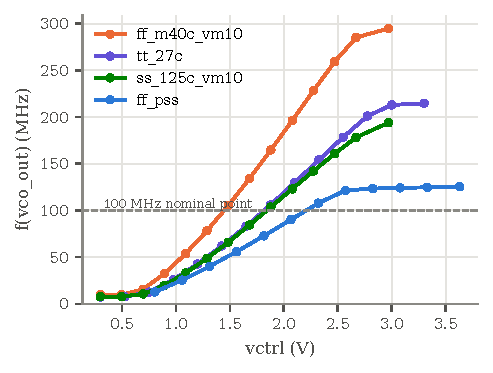
\includegraphics[width=\columnwidth]{vco_tuning}
\caption{Post-layout VCO tuning curves (extracted netlist, $v_\text{ctrl}$
forced) at the corners with the highest (\code{ff\_m40c\_vm10}) and lowest
(\code{ff\_pss}) ceiling, at typical, and at slow-hot-low-supply. The
flattening at the top is the bias-tracking ceiling. \code{ff\_pss} reaches \SI{100}{MHz} at $v_\text{ctrl}\approx\SI{2.2}{V}$, where the closed loop settles at that corner (\cref{tab:cosim}). Points below about
\SI{5}{MHz} are under the bench's resolution and omitted.}
\label{fig:vco}
\end{figure}

\subsection{TSPC divide-by-2}\label{sec:tspc}
The first divider stage must toggle at whatever the VCO reaches, including
during acquisition overshoot; if it drops edges, \code{clk\_fb} looks slow,
the PFD pumps UP, and the loop runs away to the rail. At the slow corner no
library flop does this with margin: the best \code{dffrnq\_2}+\code{inv\_1}
toggle loop closed at $-0.03$ to $+0.004$\,ns of setup slack depending on
routing. We therefore placed a nine-transistor Yuan--Svensson TSPC flop
\cite{yuan} with $D=\overline{Q}$ inside the analog macro. Three dynamic
stages (precharge on clock low, evaluate on the rising edge) toggle the
output node on each rising edge of \code{vco\_out}; a weak PMOS gated by
\code{pll\_en} holds the dynamic node high in standby so the cell is fully
static there, and two inverters buffer the result to the \code{vco\_div2}
pin. All 14 devices use $L=\SI{0.28}{\micro m}$. \Cref{fig:tspc} shows its
output at the typical corner.

\begin{figure}[t]
\centering
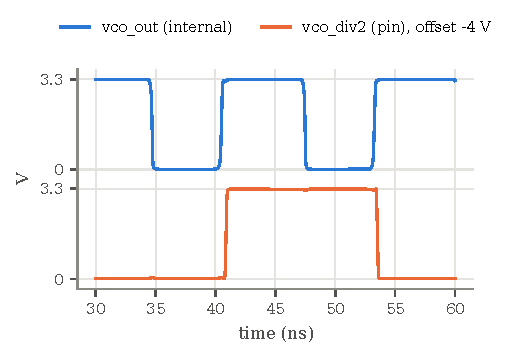
\includegraphics[width=\columnwidth]{tspc_wave}
\caption{The TSPC divider on the extracted netlist (\code{tt\_27c},
$v_\text{ctrl}=\SI{1.6}{V}$): \code{vco\_out} and the divided
\code{vco\_div2}, which toggles on every rising edge.}
\label{fig:tspc}
\end{figure}

\begin{figure*}[t]
\centering
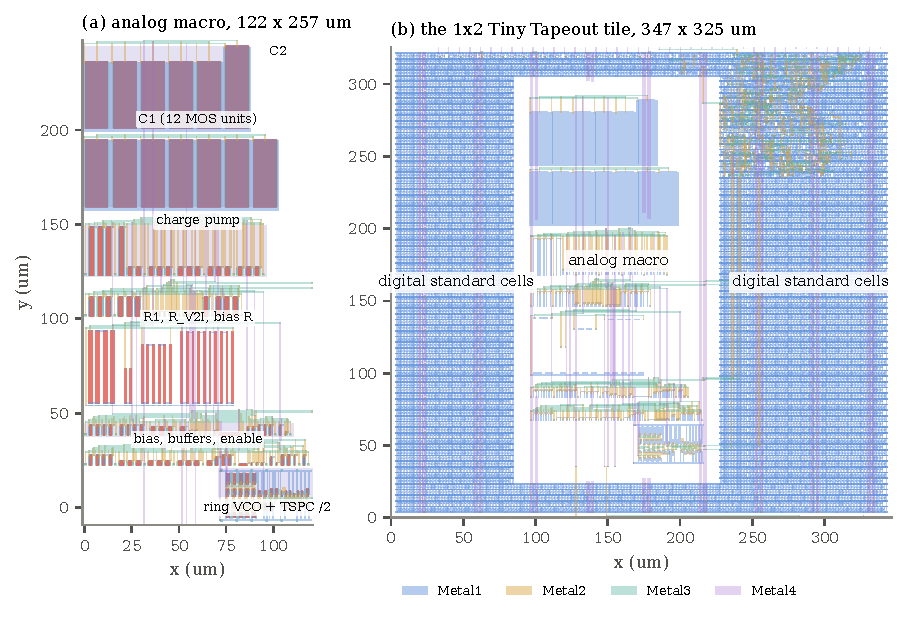
\includegraphics[width=\textwidth]{layout}
\caption{(a) The analog macro as drawn by its generator. (b) The full tile:
the analog macro in the middle, the standard-cell digital half on both
sides, and the Metal4 power straps.}
\label{fig:layout}
\end{figure*}

\section{Digital design}\label{sec:digital}
The digital half is synthesised RTL, 110 cells before placement
(\SI{3710}{\micro m^2}).
\begin{itemize}\setlength\itemsep{1pt}
\item \textbf{PFD}: two reset flops clocked by \code{clk} and \code{clk\_fb};
an AND of both outputs resets them through a delay, so both pump switches
are on together for a short pulse every cycle, which removes the dead zone.
\item \textbf{Prescaler}: two ripple toggle flops divide \code{vco\_div2} by 4
(VCO/8); a third gives VCO/16 for observation.
\item \textbf{Divider}: $N=1..5$ from \code{ui[2:0]}; unsupported codes decode
as $N=1$ so the divider never stalls.
\item \textbf{Lock detector}: a UP or DN pulse still high at the falling
edge of the reference is ``wide''; \code{LOCK} rises after 16 consecutive
reference cycles without one and falls on the next.
\item \textbf{Runaway recovery}: if the loop is enabled and unlocked for 1024
reference cycles, DN is forced for 128 cycles, pulling $v_\text{ctrl}$ to
ground. The window (\SI{82}{\micro s} at \SI{12.5}{MHz}) exceeds the
\SI{50}{\micro s} lock-time bound, so it never interrupts a normal
acquisition.
\end{itemize}
Verification: line and toggle coverage are \SI{100}{\%} (122/122 lines,
188/188 toggles); six safety properties (divider ratio, prescaler ratio,
PFD reset and no-overlap, lock behaviour, asynchronous reset) hold to depth
20 with eight cover points reached; all 16 non-equivalent RTL mutants are
killed by the testbench; and gate-level simulation of the hardened netlist
passes.

\begin{figure*}[t]
\centering
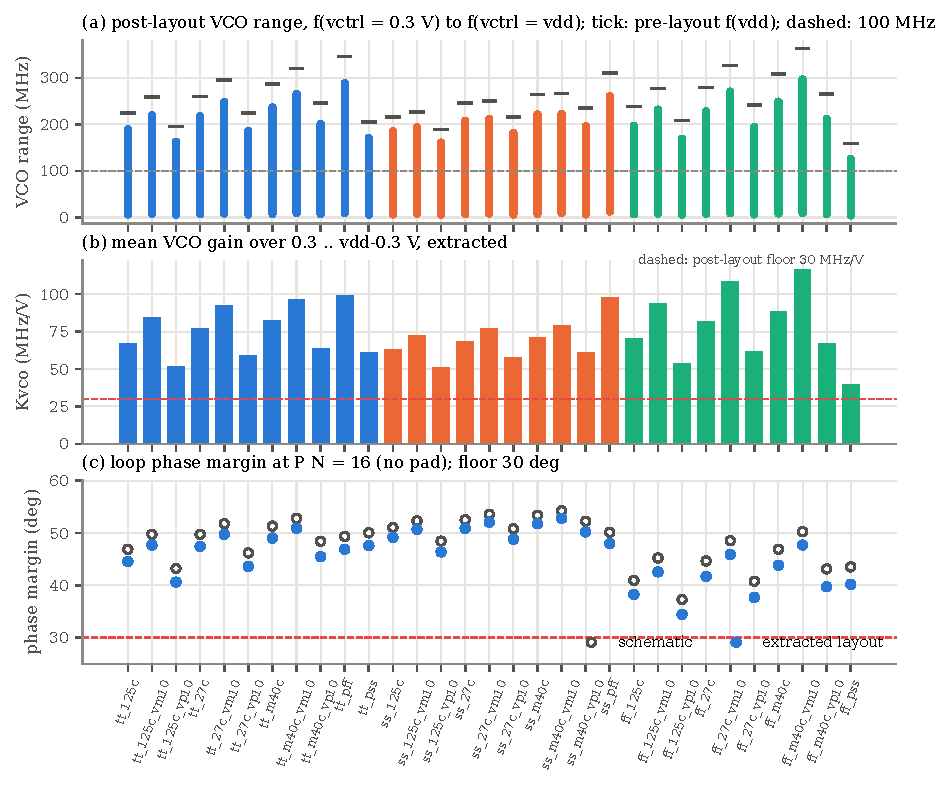
\includegraphics[width=\textwidth]{corners}
\caption{Post-layout results at all 31 corners, coloured by transistor
process (blue tt, orange ss, green ff). (a) VCO range from
$v_\text{ctrl}=\SI{0.3}{V}$ to $V_{DD}$; ticks mark the schematic's
ceiling. (b) Mean VCO gain. (c) Phase margin at $PN = 16$ from each
corner's extracted $I_{cp}$, $K_\text{vco}$ and filter impedance.}
\label{fig:corners}
\end{figure*}

\section{Loop dynamics}\label{sec:loop}
With the PFD and pump modelled in the continuous-time approximation, the
open-loop gain is
\begin{equation}
H(s) = \frac{I_{cp}}{2\pi}\,\frac{K_\text{vco}}{s}\,\frac{Z(s)}{PN},
\end{equation}
and the second-order approximation gives
$\omega_n = \sqrt{I_{cp}K_\text{vco}/(PN\,C_1)}$ and
$\zeta = \tfrac{R_1}{2}\sqrt{I_{cp}K_\text{vco}C_1/(PN)}$.
With the values calibrated from the transistor-level cell at the
\SI{100}{MHz} point ($I_{cp}=\SI{18.8}{\micro A}$, local
$K_\text{vco}=\SI{116}{MHz/V}$), the loop at $PN=16$ crosses over at
\SI{585}{kHz}, about $f_\text{ref}/10.7$, safely below the
sampling limit \cite{gardner}, with \SI{52.6}{\degree} of phase margin,
$f_n=\SI{416}{kHz}$ and $\zeta=0.71$ (\cref{fig:bode}). Phase margin falls
with $PN$ (\SI{55}{\degree} at 8, \SI{40}{\degree} at 40) because the
crossover moves down toward the zero. A \SI{5}{pF} pad on $v_\text{ctrl}$
adds to $C_2$ and costs \SIrange{10}{16}{\degree} on the extracted cell; since the pad is always
connected, \cref{sec:results} tests the loop with it.

\begin{figure}[t]
\centering
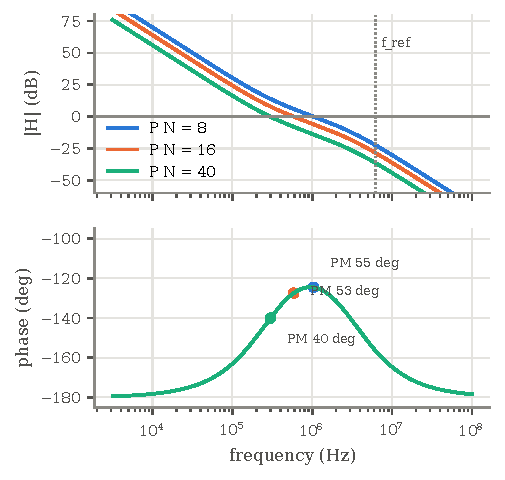
\includegraphics[width=\columnwidth]{bode}
\caption{Open-loop gain and phase from the linear model, calibrated at
\code{tt\_27c} and \SI{100}{MHz}, for three $PN$. Dots: crossover.}
\label{fig:bode}
\end{figure}

\section{Physical design}\label{sec:phys}
The analog layout is written as code (a gdsfactory/KLayout generator,
\code{gen\_pll\_analog.py}); nobody edits the GDS. Bottom to top
(\cref{fig:layout}a): the ring VCO with the TSPC beside its output
inverter, the bias, buffer and enable rows, the poly resistor serpentines,
the pump with its PMOS mirror bank, and the MOS-capacitor rows. The macro
is $122\times\SI{257}{\micro m}$; every routed internal net is labelled so
Magic's extraction keeps its coupling capacitance. It is DRC-clean (Magic
and KLayout) and LVS-matches the schematic (Netgen, unique match).

The digital half is placed and routed around the macro by LibreLane into
the $1\times2$ tile (\cref{fig:layout}b; 2350 instances including fill and
taps). The VCO-derived clock is constrained per process at twice the
extracted VCO's ceiling period plus margin (\SI{7.5}{ns} at ss,
\SI{5.4}{ns} at tt and ff) with \SI{0.20}{ns} of jitter-derived setup
uncertainty. Every STA corner meets setup and hold with no waiver
(\cref{fig:sta}); before the TSPC, the slow corner's first stage closed
within a few picoseconds at best. The tile passes full-chip DRC (Magic 0,
KLayout 0), LVS and all 12 Tiny Tapeout precheck checks.


\begin{figure}[t]
\centering
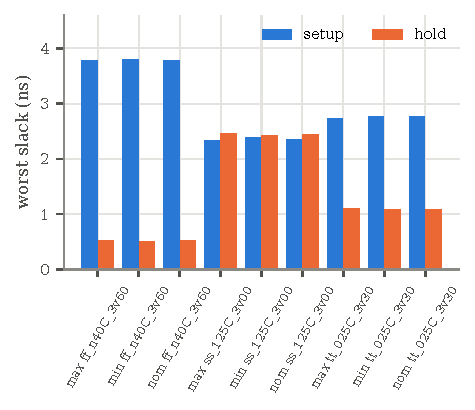
\includegraphics[width=\columnwidth]{sta}
\caption{Worst setup and hold slack of the hardened digital half at the
nine STA corners (min/nom/max parasitics $\times$ ss/tt/ff libraries).}
\label{fig:sta}
\end{figure}

\section{Results}\label{sec:results}

\subsection{PVT behaviour before and after layout}
The analog benches run at 31 corners: tt, ss and ff transistors at
\SI{-40}{}, \SI{27}{} and \SI{125}{\celsius} and $V_{DD} = 3.3\,\text{V}\pm
\SI{10}{\%}$, plus four resistor-skew corners (\code{ss\_pff},
\code{ff\_pss}, \code{tt\_pss}, \code{tt\_pff}) where transistors and
passives move in opposite directions. \Cref{fig:corners} summarises the
extracted netlist; \cref{tab:summary} gives the ranges.


\begin{table}[t]
\centering
\caption{Summary over the 31 PVT corners (post-layout unless marked).}
\label{tab:summary}
\small
\setlength\tabcolsep{4pt}
\begin{tabular}{@{}lccc@{}}
\toprule
Quantity & min & typ. & max \\
\midrule
$I_{cp}$, code 00 (\si{\micro A}) & 13.6 & 18.6 & 26.6 \\
$f_\text{vco}$ at $v_\text{ctrl}=\SI{0.3}{V}$ (MHz) & 4.5 & 7.4 & 12.9 \\
$f_\text{vco}$ at $v_\text{ctrl}=V_{DD}$ (MHz) & 126 & 217 & 297 \\
mean $K_\text{vco}$ (MHz/V) & 39.8 & 77.0 & 116.7 \\
phase margin, $PN=16$ (deg) & 34.5 & 47.4 & 52.8 \\
UP/DN mismatch (\%), sch. & 3.6 & 5.0 & 8.7 \\
overlap charge (fC), sch. & 2.0 & 2.4 & 3.6 \\
standby (\si{\micro A}), sch. & \num{1e-4} & \num{1.5e-4} & 0.026 \\
start-up (\si{\micro s}), sch. & 0.44 & 0.68 & 0.92 \\
\bottomrule
\end{tabular}
\end{table}

Layout lowers the VCO's ceiling by 14--21\,\% (the ring nodes pick up wiring
capacitance) and the phase margin by \SIrange{1.4}{3.4}{\degree}. The
binding corner is \code{ff\_pss}: fast transistors with slow resistors cut
$I_b$ by about a third, and with it the VCO ceiling (\SI{126}{MHz}),
$K_\text{vco}$ (\SI{39.8}{MHz/V}) and $I_{cp}$ (\SI{13.6}{\micro A}).
Every corner still reaches the \SI{100}{MHz} point. The lowest phase
margin, \SI{34.5}{\degree} at \code{ff\_125c\_vp10}, clears the
\SI{30}{\degree} floor.

\subsection{Closed loop on the extracted netlist}
The decisive test runs the whole loop in a mixed-signal co-simulation:
ngspice simulates the extracted analog macro at a PDK corner, temperature
and supply, while Icarus Verilog simulates the hardened gate-level digital
netlist with an SDF of the same process at the nearest characterised
temperature, the two coupled by cocotbext-ams at a \SI{0.25}{ns}
synchronisation grid. The SDFs for \SI{125}{\celsius} ff and
\SI{-40}{\celsius} ss, which the flow does not write, were generated from
the same netlist, constraints and extracted parasitics; the same script
reproduces a flow-written SDF to within \SI{1}{ps}. Two mismatches remain: the
\SI{27}{\celsius} \code{ff\_pss} uses \SI{-40}{\celsius} delays, the nearest
available, and the libraries tie voltage to process (ff \SI{3.6}{V}, ss
\SI{3.0}{V}), so the digital delays do not follow the analog corner's
supply. The corners are the
four that bound the post-layout sweep: the lowest and highest VCO ceiling
(\code{ff\_pss}, \code{ff\_m40c\_vm10}) and the lowest and highest phase
margin (\code{ff\_125c\_vp10}, \code{ss\_m40c\_vm10}). Each corner
simulates \SI{30}{\micro s} in about 40 minutes.

\begin{figure}[t]
\centering
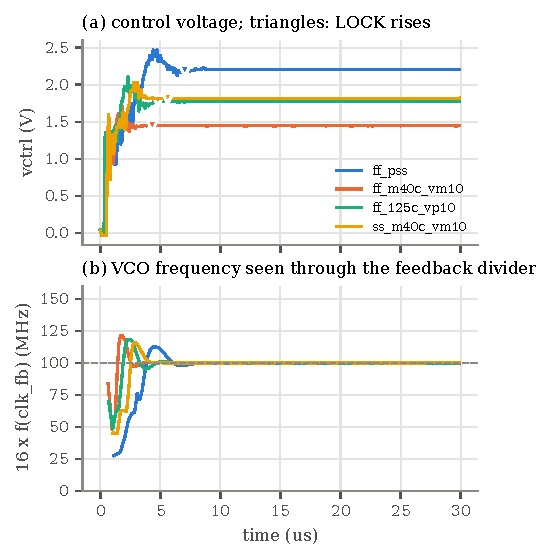
\includegraphics[width=\columnwidth]{lock}
\caption{Lock acquisition at the four bounding corners (extracted analog,
gate-level digital with SDF): (a) $v_\text{ctrl}$ with the instant
\code{LOCK} rises; (b) the VCO frequency inferred from successive
\code{clk\_fb} periods.}
\label{fig:lock}
\end{figure}

\begin{table}[t]
\centering
\caption{Closed loop at \SI{100}{MHz} ($6.25\,\text{MHz}\times16$),
extracted analog + gate-level digital. Bounds: lock $\le\SI{50}{\micro s}$,
frequency error $\le 10^{-3}$, $v_\text{ctrl}$ p-p $\le\SI{20}{mV}$.}
\label{tab:cosim}
\small
\setlength\tabcolsep{4pt}
\begin{tabular}{@{}lcccc@{}}
\toprule
Corner & lock & $f_\text{vco}$ & $v_\text{ctrl}$ & p-p \\
 & (\si{\micro s}) & (MHz) & (V) & (mV) \\
\midrule
\code{ff\_pss}        & 6.72 & 99.9998 & 2.20 & 2.4 \\
\code{ff\_m40c\_vm10} & 4.00 & 100.0009 & 1.45 & 7.2 \\
\code{ff\_125c\_vp10} & 4.96 & 100.0010 & 1.78 & 13.5 \\
\code{ss\_m40c\_vm10} & 5.12 & 100.0015 & 1.81 & 9.1 \\
\bottomrule
\end{tabular}
\end{table}

\Cref{fig:lock} and \cref{tab:cosim} show the result. The loop locks within
\SI{6.72}{\micro s} at every corner, \code{LOCK} never drops, and the VCO
settles to within $2\times10^{-5}$ of \SI{100}{MHz}. The acquisition overshoots
to about \SI{120}{MHz} at the fast corners, well inside what the TSPC and
the /4 prescaler can follow. \code{ff\_pss}, with the lowest loop gain, is
the slowest and least damped, as the model predicts; it settles with
$v_\text{ctrl}$ at \SI{2.2}{V}, the highest of the four, because its VCO is
the slowest. The static phase offset is \SIrange{0.87}{1.14}{ns} at the ff corners and
\SI{2.3}{ns} at \code{ss\_m40c\_vm10}: the PFD's reset pulse plus pump
mismatch. Timing the digital half by process alone, as a first run did,
gave \code{ff\_125c\_vp10} \SI{3.5}{mV} and \code{ss\_m40c\_vm10}
\SI{15.9}{mV} of ripple, so the ripple depends on the digital delays and
these figures should not be read more finely than that.

\begin{figure}[t]
\centering
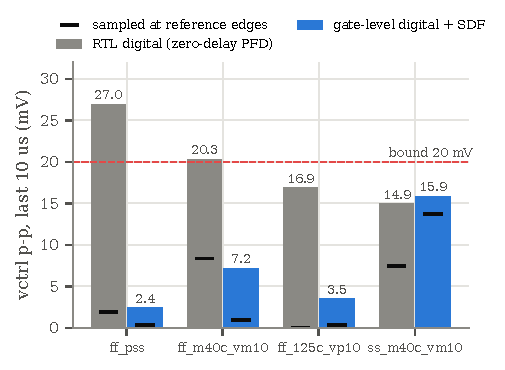
\includegraphics[width=\columnwidth]{settle}
\caption{Ripple on $v_\text{ctrl}$ over the last \SI{10}{\micro s},
sampled every \SI{5}{ns}, with the RTL digital and with the gate-level
digital. Ticks: the same signal sampled at reference edges only.}
\label{fig:settle}
\end{figure}

\subsection{Why the gate-level digital matters}
Running the same bench with the RTL in place of the gate-level netlist
locks just as well, but leaves 27.0 and \SI{20.3}{mV} of peak-to-peak
ripple on $v_\text{ctrl}$ at \code{ff\_pss} and \code{ff\_m40c\_vm10}
(\cref{fig:settle}). The cause is the RTL PFD's zero-delay reset: it never
turns both pumps on together, so whatever phase error remains, rounded to
the synchronisation grid, is corrected by one pump firing alone, and that
lone current through $R_1$ appears as a spike of
$I_{cp}R_1 \approx \SI{0.5}{V}$ filtered by $C_2$. Sampled at reference
edges, the RTL's $v_\text{ctrl}$ moves only 0.03--\SI{8}{mV}. The
gate-level PFD has a real reset delay, so both pumps overlap briefly every
cycle, the correction is a small difference of two currents, and the
ripple falls to 2.4--\SI{13.5}{mV}. The lesson is that a zero-delay PFD is fine for checking
lock but misleading for ripple and spurs, which depend on the reset
pulse.

\subsection{With the control-pad load}
$v_\text{ctrl}$ reaches pad \code{ua[0]}, so the pad's capacitance is on the
loop in any real package, probe or no probe. The runs above leave it out.
Repeating them with \SI{5}{pF} from $v_\text{ctrl}$ to ground inside the
extracted cell, at the four corners and \code{tt\_27c}, all five lock within
\SI{7.5}{\micro s} (\SI{0.2}{}--\SI{1.0}{\micro s} later than without), hold,
and meet every bound; the pad filters the pump's spikes, leaving
0.8--\SI{4.5}{mV} of ripple (\cref{fig:pad}). The cost is margin:
small-signal phase margin on the extracted cell with the same pad falls to
\SI{23.9}{\degree} at \code{ff\_125c\_vp10}, and 9 of the 31 corners are
below the \SI{30}{\degree} floor the no-pad loop is held to. The time-domain
runs show this loop stable, not that this margin is comfortable, and
\SI{5}{pF} is the specification's allowance rather than a measured pad.

\begin{figure}[t]
\centering
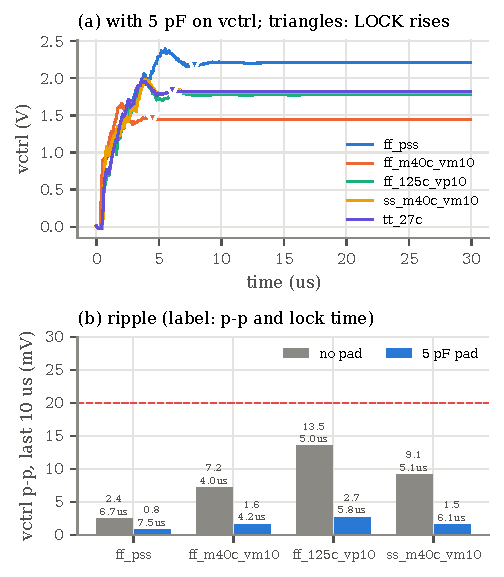
\includegraphics[width=\columnwidth]{pad}
\caption{With \SI{5}{pF} on $v_\text{ctrl}$ (extracted analog, gate-level
digital): (a) acquisition, (b) ripple with and without the pad.}
\label{fig:pad}
\end{figure}

\subsection{Other divider settings and re-lock}
A second bench changes $N$ while the loop runs, at $f_\text{ref}=\SI{5}{MHz}$:
$N=1\to3\to2$ (\SI{40}{}, \SI{120}{}, \SI{80}{MHz}), \SI{20}{\micro s} each,
at the four corners and \code{tt\_27c} (\cref{fig:cov}a). Four corners lock
at every setting to within \num{1e-4}, re-locking within
\SI{5.2}{\micro s}. \code{ff\_pss} does not: \SI{120}{MHz} is close to its
\SI{125.6}{MHz} ceiling, where $K_\text{vco}$ collapses, so the step drives
$v_\text{ctrl}$ to \SI{3.5}{V}, above the \SI{3.3}{V} supply, before it comes
back. \code{LOCK} pulses for \SI{1.6}{\micro s} on the way down, then rises
for good \SI{15}{\micro s} after the step, and the last \SI{4}{\micro s} of
the segment still moves \SI{229}{mV}. Given longer it settles: to
\SI{20}{mV} about \SI{25}{\micro s} after the step (\cref{fig:cov}b), and the
same holds with the pad and when acquiring \SI{120}{MHz} directly from enable.
So \code{LOCK} near a corner's ceiling does not by itself mean the frequency
has settled.

These segments are not held to the \SI{100}{MHz} point's \SI{20}{mV} ripple
bound, and some would miss it: up to \SI{24.8}{mV} at \code{tt\_27c} in the
\SI{4}{\micro s} window. With the pad at \code{ff\_125c\_vp10} the same
steps pass, and the top of the reference range ($\SI{12.5}{MHz}\times8$,
\code{tt\_27c}) locks in \SI{3.8}{\micro s}. The largest $PN$ in reach at the lowest-margin corner, $N=4$ (\SI{160}{MHz},
\SI{169}{MHz} ceiling) with the pad, overshoots to \SI{3.3}{V} and rings: not
settled in \SI{30}{\micro s} by the \num{1e-3} frequency bound, but within
\SI{20}{mV} by \SI{27}{\micro s} and \SI{3}{mV} p-p, $10^{-5}$ off, by the end of an
\SI{80}{\micro s} run.

\begin{figure}[t]
\centering
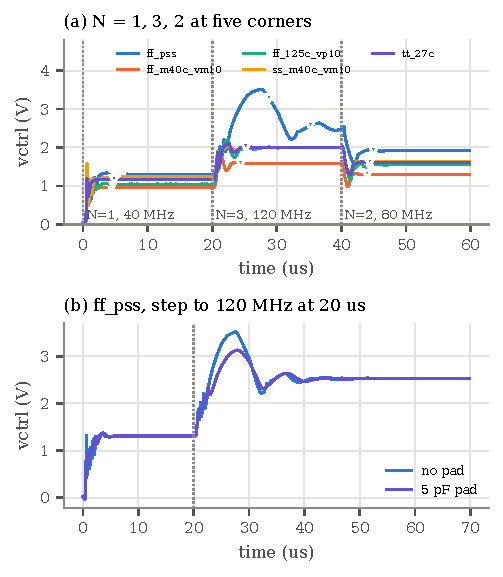
\includegraphics[width=\columnwidth]{cov}
\caption{Divider steps at $f_\text{ref}=\SI{5}{MHz}$: (a) $v_\text{ctrl}$
at five corners (triangles: \code{LOCK} rises); (b) the \SI{120}{MHz} step at
\code{ff\_pss} given \SI{50}{\micro s}, with and without the pad.}
\label{fig:cov}
\end{figure}

\section{Discussion and limitations}\label{sec:disc}
\textbf{What this shows.} The evidence is simulation only. It supports
``implemented, and demonstrated to lock in post-layout mixed-signal
simulation''. It does not support ``silicon-proven'' or ``low-jitter''.

\textbf{Lock range.} After layout the VCO covers about
\SIrange{13}{125}{MHz} at every corner (\SIrange{7}{217}{MHz} at typical),
so the datasheet promises only the guaranteed range; the slow-resistor
corner sets the top.

\textbf{Jitter} is estimated, not measured. ngspice has no device transient
noise, so noise sources sized from each device's model at its bias
(white and $1/f$) are injected into the extracted cell, except the output
buffer and divider. At the \SI{100}{MHz} point, over two or three seeds of 520
periods, free-running period jitter is \SI{9.7}{ps} rms at \code{tt\_27c},
\SI{10.2}{ps} at \code{ss\_125c\_vm10} and \SI{13.5}{ps} at
\code{ff\_125c\_vm10}, the highest of the nine corners run (six of them
in shorter screening runs; the other 22 were not run). A deterministic
alternation of up to $\pm\SI{6.8}{ps}$ on the output is separate from these
figures. They replace a first estimate of
1.2--\SI{2.5}{ps}, which came from 30--36 periods at the top of the VCO's range
with less of the noise included. For the locked output we have only a linear
model, not a simulation: from the simulated VCO phase noise and $R_1$'s thermal
noise it gives 44--\SI{61}{ps} rms from \SI{10}{kHz} to \SI{50}{MHz} at those
three corners, or 35--\SI{43}{ps} without the VCO's $1/f$ term, whose level is
uncertain by a factor of 2--4 in power. It leaves out reference, PFD,
charge-pump and supply noise, so it does not bound the jitter of a real chip.
The STA's \SI{0.20}{ns} setup uncertainty was derived from the first estimate;
it still covers $7\sigma$ of the worst figure across the two VCO periods of
\code{vco\_div2} (about \SI{155}{ps}), but with far less room, and jitter at the
faster clock the STA is constrained to was not simulated. Nothing here
measures reference spurs or supply noise.

\textbf{Device mismatch.} The specification had excluded Monte Carlo on the
belief that the PDK models carry no per-instance mismatch. They do, for MOS
devices. On the schematic, 200 samples per corner put the worst-case UP/DN
pump mismatch over its \SI{10}{\%} bound in 26\,\% of samples at \code{ff\_pss}
(95\,\% interval 20--33\,\%; worst \SI{14.6}{\%}) and 6\,\% at
\code{ff\_m40c\_vp10}, and in none at \code{ss\_pff} or \code{tt\_27c}. The
peak is at the edge of the $v_\text{ctrl}$ range. So the row in
\cref{tab:summary} is the spread with statistics off. At \code{tt\_27c} the
overlap charge (worst \SI{3.4}{fC}, bound \SI{10}{fC}) and bias start-up hold;
the VCO frequency at mid-range is \SI{101.7}{MHz} with $\sigma=\SI{2.5}{MHz}$.
These are rates given a corner, not a product yield, and they leave out layout
gradients, resistor mismatch (the models have none) and capacitor variation;
Kvco and phase margin were not run. Closed-loop runs with one pump source widened by about $3\sigma$ (extracted cell
and gate-level digital at \SI{100}{MHz}; UP \SI{+6}{\%} reads \SI{14.2}{\%} on the
same DC sweep at \code{ff\_pss}, UP \SI{+5}{\%} reads \SI{12.1}{\%} at
\code{ff\_m40c\_vp10}) all lock and hold. $v_\text{ctrl}$ ripple is \SIrange{1.0}{2.5}{mV}
at \code{ff\_pss} against \SI{2.4}{mV} unskewed, and \SIrange{3.3}{6.3}{mV} at
\code{ff\_m40c\_vp10} against \SI{5.4}{mV}, inside the \SI{20}{mV} bound; the static phase
offset stays between 0.44 and \SI{0.98}{ns}. So we keep the \SI{10}{\%} bound as written and do not
resize the pump, since at this operating point a pump over that bound does not hurt the loop.
This is a widened device, not a drawn sample, at one divider setting; a pump skew during
an N step and at the pad-loaded corners was not run.

\textbf{Coverage of the closed-loop tests.} The extracted loop has been run
at five corners, not 31, and at the settings above. The 31-corner sweep
characterises analog behaviour; it does not demonstrate acquisition at every
corner and setting. $N=5$ has not been run on the extracted netlist, and $N=4$ only at one corner.

\textbf{Bench strength.} A mutation check of the analog benches (each
device's width and length doubled or halved) flags mutants that move no
measure beyond the run-to-run spread. After the TSPC change it found one
new mutant just under the \SI{2}{\%} floor, and the TSPC's own 14 devices
are not yet in the mutated set; both await the owner's ruling.

\section{Conclusion}
A complete charge-pump PLL---bias, pump, MOS-capacitor filter, ring VCO,
TSPC prescaler and standard-cell control---fits one $1\times2$ GF180 Tiny
Tapeout tile and is DRC, LVS and precheck clean. Moving the first divide
stage into the analog macro as a TSPC flop turned a timing closure measured
in picoseconds into \SI{2.3}{ns} of margin. With parasitics extracted and
the real gate-level digital in the loop, the PLL locks to \SI{100}{MHz} in
under \SI{7}{\micro s} with at most \SI{14}{mV} of control ripple at every
corner that bounds its range, and it stays stable with the control pad's
load. It has not been fabricated; the phase margin with the pad, settling near
the VCO's ceiling, jitter and pump mismatch are the risks to check first.

\section*{Reproducing this paper}
\small All results are recorded in the repository with hashes of their
inputs. \code{docs/paper/sims/} re-runs the two post-layout ngspice
benches behind \cref{fig:vco,fig:tspc}; \code{docs/paper/make\_figs.py}
redraws every figure; \code{make -C docs/paper} builds this PDF.
\code{blocks/pll/tb/README.md} explains the co-simulation benches, and
\code{blocks/pll/tb/gl/} holds the gate-level netlist, parasitics and SDFs
those runs read.

\begin{thebibliography}{9}\small
\bibitem{gardner} F.~M. Gardner, ``Charge-pump phase-lock loops,''
\emph{IEEE Trans. Commun.}, vol.~28, no.~11, pp.~1849--1858, 1980.
\bibitem{razavi} B.~Razavi, \emph{Design of CMOS Phase-Locked Loops}.
Cambridge University Press, 2020.
\bibitem{yuan} J.~Yuan and C.~Svensson, ``High-speed CMOS circuit technique,''
\emph{IEEE J. Solid-State Circuits}, vol.~24, no.~1, pp.~62--70, 1989.
\end{thebibliography}
\end{document}
